\section{Deep learning}

\newcommand{\polynomialplot}[1]{
    \begin{tikzpicture}
        \begin{axis}[
            height=6cm,
            width=6cm,
            xmin=-1.6,
            xmax=1.6,
            ymin=0,
            ymax=5,
            xmajorticks=false,
            ymajorticks=false,
            xlabel=$x$,
            ylabel=$y$
        ]
            \addplot[
                samples=100,
                domain=-1.6:1.6,
                only marks,
                blue,
                opacity=0.5
            ] (x, {x^4-3*x^2-x+4+0.5*rand});

            \ifnum#1=1
                \addplot[
                    samples=100,
                    domain=-1.6:1.6,
                    red,
                    very thick
                ] (x, {x^4-3*x^2-x+4});
            \fi
            \ifnum#1=2
                \addplot[
                    samples=100,
                    domain=-1.6:1.6,
                    red,
                    very thick
                ] coordinates {
                    (-1.6, 4.4)
                    (-1.4, 4.4)
                    (-1.4, 3)
                    (-0.8, 3)
                    (-0.8, 4)
                    (0.2, 4)
                    (0.2, 3)
                    (0.6, 3)
                    (0.6, 2)
                    (0.8, 2)
                    (0.8, 0.8)
                    (1.6, 0.8)
                };
            \fi
            \ifnum#1=3
                \addplot[
                    samples=100,
                    domain=-1.6:1.6,
                    red,
                    very thick
                ] (x, {x^4-3*x^2-x+4+0.1*rand});
            \fi
            \ifnum#1=4
                \addplot[
                    samples=100,
                    domain=-1.6:1.6,
                    red,
                    very thick
                ] coordinates {
                    (-1.6, 4.4)
                    (-1.4, 3)
                    (-1.3, 2.9)
                    (-1.1, 2.9)
                    (-0.5, 3.8)
                    (0, 3.8)
                    (0.4, 3)
                    (1, 1)
                    (1.2, 0.7)
                    (1.6, 1.2)
                };
            \fi
            \ifnum#1=5
                \addplot[
                    samples=100,
                    domain=-1.6:1.6,
                    red,
                    very thick
                ] coordinates {
                    (-1.6, 4.4)
                    (-1.4, 3)
                    (-1.3, 2.9)
                    (-1.1, 2.9)
                    (-0.5, 3.8)
                    (0, 3.8)
                    (0.4, 3)
                    (1, 1)
                    (1.2, 0.7)
                    (1.6, 1.2)
                };

                \addplot[
                    samples=100,
                    domain=-1.6:1.6,
                    orange,
                    very thick
                ] (x, {x^4-3*x^2-x+4});
            \fi
        \end{axis}
    \end{tikzpicture}
}

\newsavebox{\polynomialdata}
\sbox{\polynomialdata}{
    \polynomialplot{0}
}
\newsavebox{\polynomialspline}
\sbox{\polynomialspline}{
    \polynomialplot{1}
}
\newsavebox{\polynomialtree}
\sbox{\polynomialtree}{
    \polynomialplot{2}
}
\newsavebox{\polynomialpiecewise}
\sbox{\polynomialpiecewise}{
    \polynomialplot{3}
}
\newsavebox{\polynomialapprox}
\sbox{\polynomialapprox}{
    \polynomialplot{4}
}
\newsavebox{\polynomialboth}
\sbox{\polynomialboth}{
    \polynomialplot{5}
}

\newsavebox{\correlatedpredictors}
\sbox{\correlatedpredictors}{
    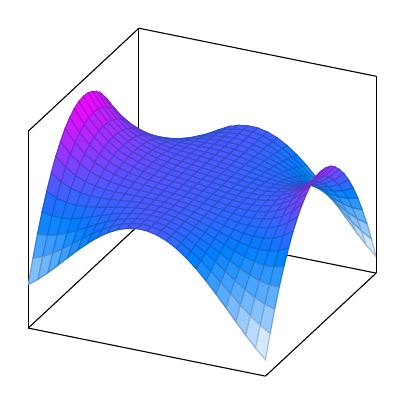
\begin{tikzpicture}
        \begin{axis}[
            height=6cm,
            width=6cm,
            xmajorticks=false,
            ymajorticks=false,
            zmajorticks=false
        ]
            \addplot3 [
                surf,
                domain=-1.5:1.5,
                y domain=-1.5:1.5,
                colormap/cool,
                draw=black
            ] {{x^4-3*(x*y)^2-x+4}};
        \end{axis}
    \end{tikzpicture}
}
\begin{frame}{Deep learning: Motivation}
    \begin{tikzpicture}
        \node[] at (-5.25, 3.5) {};
        \node[] at (5.25, -3.5) {};

        \visible<1,6>{
            \node[] at (0, 0.5) {
                \usebox{\polynomialdata}
            };
        }
        %shader=interp,
        \visible<2>{
            \node[] at (0, 0.5) {
                \usebox{\polynomialspline}
            };
            \node[font=\small] at (0, -2.75) {
                $\hat{y}=s(x)$
            };
        }
        \visible<3>{
            \node[] at (0, 0.5) {
                \usebox{\polynomialtree}
            };
            \node[font=\small] at (0, -2.75) {
                $\hat{y}=
                \begin{cases}
                    4&\cdots\\
                    3&0.2\leq x<0.6\\
                    1.5&\cdots\\
                \end{cases}
                $
            };
        }
        \visible<4>{
            \node[] at (0, 0.5) {
                \usebox{\correlatedpredictors}
            };
        }
        \visible<5>{
            \node[inner sep=0pt, draw=black] at (-2.5, 0) {
                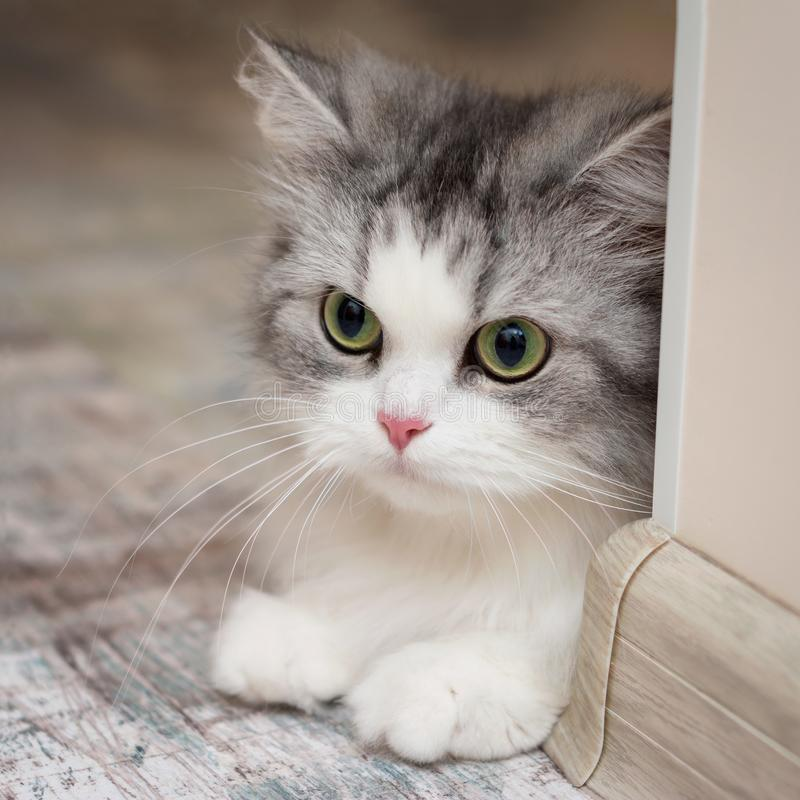
\includegraphics[width=3cm]{data/cat.png}
            };
            \node[align=center, draw=black] at (2.5, 0) {
                The cat wagged\\ its tail
            };
        }
        \visible<7>{
            \node[] at (0, 0.5) {
                \usebox{\polynomialpiecewise}
            };
        }
    \end{tikzpicture}
\end{frame}

\newsavebox{\threedimensional}
\sbox{\threedimensional}{
    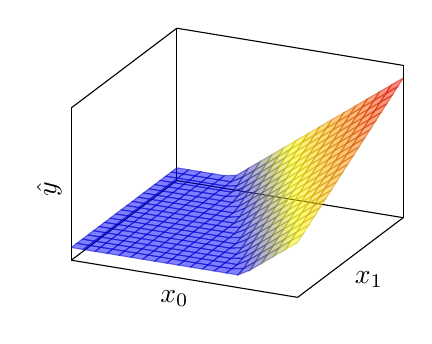
\begin{tikzpicture}[
        declare function = {
            q(\x) = \x - 1;
            Z(\x,\y) = max(0, \x*0.5 + \y*0.25);
        }
    ]
        \begin{axis}
        [
            height=5cm,
            ticks=none,
            xlabel=$x_0$,
            ylabel=$x_1$,
            zlabel=$\hat{y}$,
            domain=-1:1,
            samples=20,
        ]
            \addplot3 [surf, opacity=0.5] {Z(x,y)};
        \end{axis}
    \end{tikzpicture}
}

\newcommand{\examplefunction}[1]{
    \begin{tikzpicture}
        \begin{axis}[
            height=4cm,
            width=10cm,
            ticklabel style={font=\footnotesize},
            xlabel=\footnotesize{$x$},
            ylabel=\footnotesize{$\hat{y}$},
            xmin=-2,
            xmax=2,
            xtick pos=bottom,
            ytick pos=left
        ]
            \ifnum#1=0
                \addplot[
                    domain=-2:2,
                    samples=100,
                    thick,
                    red
                ] (x, {max(0, max(0, -2*x+3) - 4*max(0, 5*x-6)+7)});
            \fi
            \ifnum#1=1
            \addplot[
                domain=-2:2,
                samples=100,
                thick,
                red
            ] (x, {max(0, -7*max(0, 6*x-5) +4*max(0, -3*x+2)-1)});
            \fi
        \end{axis}
    \end{tikzpicture}
}

\newsavebox{\firstexample}
\sbox{\firstexample}{
    \examplefunction{0}
}

\newsavebox{\secondexample}
\sbox{\secondexample}{
    \examplefunction{1}
}


\begin{frame}{Deep learning: Artificial neural networks}
    \centering
    \begin{tikzpicture}
        \node[] at (-5, 3) {};
        \node[] at (5, -4.5) {};

        \visible<1>{
            \artificialneuron{(0, 1.5)}{n}{0}
            \node[] (x) at (-1.5, 1.5) {$x$};
            \node[] (b) at (0, 2.5) {$\beta_0$};
            \node[] (y) at (1.5, 1.5) {$\hat{y}$};

            \draw[->] (x) -- (n) node [midway, above] {$\beta_1$};
            \draw[->] (b) -- (n);
            \draw[->] (n) -- (y);

            \node[] at (0, 0) {$\hat{y}=\beta_0+\beta_1x$};
        }

        \visible<2-3>{
            \node[] at (0, 0) {$\hat{y}=wx+b$};
        }
        \visible<2-5>{
            \artificialneuron{(0, 1.5)}{n}{0}
            \node[] (x) at (-1.5, 1.5) {$x$};
            \node[] (b) at (0, 2.5) {$b$};
            \node[] (y) at (1.5, 1.5) {$\hat{y}$};

            \draw[->] (x) -- (n) node [midway, above] {$w$};
            \draw[->] (b) -- (n);
            \draw[->] (n) -- (y);
        }
        \visible<3>{
            \draw[] (-2, -1.5) -- (2, -1.5) -- (2, -4) -- (-2, -4) -- (-2, -1.5);

            \draw[very thick, blue!60] (-2, -3.5) -- (2, -1.75);

            \node[anchor=north] at (0, -4.1) {x};
            \node[anchor=south, rotate=90] at (-2.1, -2.75) {$\hat{y}$};
        }
        \visible<4>{
            \node[] at (0, 0) {$\hat{y}=\dfrac{e^{wx+b}}{1+e^{wx+b}}$};

            \node[anchor=south, font=\footnotesize\selectfont] at (0, -1.5) {Sigmoid};

            \draw[] (-2, -1.5) -- (2, -1.5) -- (2, -4) -- (-2, -4) -- (-2, -1.5);
            \draw[very thick, blue!60, smooth] (-2, -3.5) -- (-1, -3.5) to[in=180, out=0] (1, -1.75) -- (2, -1.75);

            \node[anchor=north] at (0, -4.1) {x};
            \node[anchor=south, rotate=90] at (-2.1, -2.75) {$\hat{y}$};
        }
        \visible<5>{
            \node[] at (0, 0) {$\hat{y}=max(0, wx+b)$};

            \node[anchor=south, font=\footnotesize\selectfont] at (0, -1.5) {Rectified Linear Unit (ReLU)};

            \draw[] (-2, -1.5) -- (2, -1.5) -- (2, -4) -- (-2, -4) -- (-2, -1.5);
            \draw[very thick, blue!60] (-2, -3.5) -- (0, -3.5) -- (2, -1.75);

            \node[anchor=north] at (0, -4.1) {x};
            \node[anchor=south, rotate=90] at (-2.1, -2.75) {$\hat{y}$};
        }
        \visible<6>{
            \artificialneuron{(0, 1.5)}{n}{0}

            \node[] (x0) at (-1.5, 2) {$x_0$};
            \node[] (x1) at (-1.5, 1) {$x_1$};
            \node[] (b) at (0, 2.5) {$b$};
            \node[] (y) at (1.5, 1.5) {$\hat{y}$};
            \node[] at (0, 0) {$\hat{y}=max(0, w_0x_0+w_1x_1+b)$};

            \draw[->] (x0) -- (n) node [midway, above] {$w_0$};
            \draw[->] (x1) -- (n) node [midway, below] {$w_1$};
            \draw[->] (b) -- (n);
            \draw[->] (n) -- (y);

            \node[] at (0, -2.75) {
                \usebox{\threedimensional}
            };
        }
        \visible<7>{
            \artificialneuron{(0, 2)}{n0}{0}
            \artificialneuron{(0, 1)}{n1}{0}

            \node[] (x) at (-1.5, 1.5) {$x$};
            \node[] (y) at (1.5, 1.5) {$\hat{y}$};
            \node[] at (0, 0) {$\hat{y}=max(0, w_0x+b_0)+max(0, w_1x+b_1)$};

            \draw[->] (x) -- (n0) node [midway, above] {$w_0$};
            \draw[->] (x) -- (n1) node [midway, below] {$w_1$};
            \draw[->] (n0) -- (y);
            \draw[->] (n1) -- (y);

            \draw[] (-2, -1.5) -- (2, -1.5) -- (2, -4) -- (-2, -4) -- (-2, -1.5);
            \draw[very thick, blue!60] (-2, -3.5) -- (-0.66, -3.5) -- (0.66, -2.25) -- (2, -3);

            \node[anchor=north] at (0, -4.1) {x};
            \node[anchor=south, rotate=90] at (-2.1, -2.75) {$\hat{y}$};
        }
        \visible<8>{
            \node[] at (0, 0) {
                \usebox{\polynomialapprox}
            };
            \node[] at (0, -2.5) {
                Piecewise linear function
            };
        }
        \visible<9>{
            \node[align=center, text width=10cm] at (0, -0.75) {
                \textbf{Universal approximation theorem:}\\
                \begin{quotation}
                    \centering
                    "Any relationship that can be described with a polynomial function can be approximated by a neural network with a single hidden layer."
                \end{quotation}
            };
        }
        \visible<10,12-17>{
            \artificialneuron{(0, 2)}{n00}{0}
            \artificialneuron{(0, 1)}{n01}{0}
        }
        \visible<10-12>{
            \node[
                circle,
                minimum size=\nodesize,
                inner sep=0pt,
                text depth=0
            ] (x) at (-3, 1.5) {\footnotesize{$x$}};
        }
        \visible<10-11>{
            \node[
                circle,
                minimum size=\nodesize,
                inner sep=0pt,
                text depth=0
            ] (y) at (3, 1.5) {\footnotesize{$\hat{y}$}};

            \draw[->] (x) -- (n00) node [midway, above] {$w_0$};
            \draw[->] (x) -- (n01) node [midway, below] {$w_1$};

            \draw[->] (n00) -- (y);
            \draw[->] (n01) -- (y);

            \node[anchor=north] (formula) at (0, 0) {\tiny{
                \begin{math}
                    \begin{alignedat}{5}
                        \hat{y} = max(0, w_0x+b_0)+max(0, w_1x+b_1)\\
                    \end{alignedat}
                \end{math}
            }};
        }
        \visible<11>{
            \highlightedneuron{(0, 2)}{n00}{0}{red}
            \highlightedneuron{(0, 1)}{n01}{0}{orange}
            \node[minimum height=0.4cm, minimum width=1.55cm, draw=red] at ($ (formula) - (0.64, 0) $) {};
            \node[minimum height=0.4cm, minimum width=1.55cm, draw=orange] at ($ (formula) + (1.1, 0) $) {};
        }
        \visible<13-16>{
            \node[
                circle,
                draw=black,
                fill=nodefill,
                minimum size=\nodesize,
                inner sep=0pt,
                text depth=0
            ] (x) at (-3, 1.5) {\footnotesize{$x$}};
        }
        \visible<12-14>{
            \draw[->] (x) -- (n00) node [midway, above] {$w^0_0$};
            \draw[->] (x) -- (n01) node [midway, below] {$w^0_1$};

            \draw[->] (n00) -- (y) node [midway, above] {$w^1_0$};
            \draw[->] (n01) -- (y) node [midway, below] {$w^1_1$};

            \node[anchor=north] at (0, 0) {\tiny{
                \begin{math}
                    \begin{alignedat}{5}
                        \hat{y} = max(0, w^1_0*max(0, w^0_0*x+b^0_0)+w^1_1*max(0, w^0_1*x+b^0_1)+b^1_0)\\
                    \end{alignedat}
                \end{math}
            }};
        }
        \visible<12-19>{
            \node[
                circle,
                draw=black,
                fill=nodefill,
                minimum size=\nodesize,
                inner sep=0pt,
                text depth=0
            ] (y) at (3, 1.5) {\footnotesize{$\hat{y}$}};
        }
        \visible<14>{
            \node[text depth=0] at (-3, 0.3) {\textcolor{red}{Input}};
            \node[text depth=0] at (0, 0.3) {\textcolor{red}{Hidden}};
            \node[text depth=0] at (3, 0.3) {\textcolor{red}{Output}};
        }
        \visible<15>{
            \node[] at (0, -2.5) {
                \usebox{\firstexample}
            };
            \draw[->] (x) -- (n00) node [midway, above] {$-2$};
            \draw[->] (x) -- (n01) node [midway, below] {$5$};

            \draw[->] (n00) -- (y) node [midway, above] {$1$};
            \draw[->] (n01) -- (y) node [midway, below] {$-4$};

            \node[anchor=north] at (0, 0) {\tiny{
                \begin{math}
                    \begin{alignedat}{5}
                        \hat{y} = max(0, 1*max(0, (-2)*x+3)+(-4)*max(0, 5*x+(-6))+7)\\
                    \end{alignedat}
                \end{math}
            }};
        }
        \visible<16>{
            \node[] at (0, -2.5) {
                \usebox{\secondexample}
            };
            \draw[->] (x) -- (n00) node [midway, above] {$6$};
            \draw[->] (x) -- (n01) node [midway, below] {$-3$};

            \draw[->] (n00) -- (y) node [midway, above] {$-7$};
            \draw[->] (n01) -- (y) node [midway, below] {$4$};

            \node[anchor=north] at (0, 0) {\tiny{
                \begin{math}
                    \begin{alignedat}{5}
                        \hat{y} = max(0, -7*max(0, 6*x+(-5))+4*max(0, (-3)*x+2)-1)\\
                    \end{alignedat}
                \end{math}
            }};
        }
        \visible<17-19>{
            \node[
                circle,
                draw=black,
                fill=nodefill,
                minimum size=\nodesize,
                inner sep=0pt,
                text depth=0
            ] (x0) at (-3, 2) {\footnotesize{$x_0$}};
            \node[
                circle,
                draw=black,
                fill=nodefill,
                minimum size=\nodesize,
                inner sep=0pt,
                text depth=0
            ] (x1) at (-3, 1) {\footnotesize{$x_1$}};
        }
        \visible<17>{
            \draw[->] (x0) -- (n00);
            \draw[->] (x0) -- (n01);
            \draw[->] (x1) -- (n00);
            \draw[->] (x1) -- (n01);
            \draw[->] (n00) -- (y);
            \draw[->] (n01) -- (y);

            \node[anchor=north] at (0, 0) {\tiny{
                \begin{math}
                    \begin{alignedat}{5}
                        \hat{y} &= max(0, &&w^1_{0,0}*max(0, w^0_{0,0}*x_0+w^0_{1,0}*x_{1}+b_{0,0})+\\[\spacing]
                        & &&w^1_{1,0}*max(0, w^0_{0,1}*x_0+w^0_{1,1}*x_{1}+b_{0,1})+\\[\spacing]
                        & &&b_1)&&\\
                    \end{alignedat}
                \end{math}
            }};
        }
        \visible<18>{
            \artificialneuron{(0, 2.5)}{n00}{0}
            \artificialneuron{(0, 1.5)}{n01}{0}
            \artificialneuron{(0, 0.5)}{n02}{0}

            \draw[->] (x0) -- (n00);
            \draw[->] (x0) -- (n01);
            \draw[->] (x0) -- (n02);
            \draw[->] (x1) -- (n00);
            \draw[->] (x1) -- (n01);
            \draw[->] (x1) -- (n02);

            \draw[->] (n00) -- (y);
            \draw[->] (n01) -- (y);
            \draw[->] (n02) -- (y);

            \node[anchor=north] at (0, 0) {\tiny{
                \begin{math}
                    \begin{alignedat}{5}
                        \hat{y} &= max(0, &&w^1_{0,0}*max(0, w^0_{0,0}*x_0+w^0_{1,0}*x_{1}+b_{0,0})+\\[\spacing]
                        & &&w^1_{1,0}*max(0, w^0_{0,1}*x_0+w^0_{1,1}*x_{1}+b_{0,1})+\\[\spacing]
                        & &&w^1_{2,0}*max(0, w^0_{0,2}*x_0+w^0_{1,2}*x_{1}+b_{0,2})+\\[\spacing]
                        & &&b_1)&&\\
                    \end{alignedat}
                \end{math}
            }};
        }
        \visible<19>{
            \artificialneuron{(-1, 2.5)}{n00}{0}
            \artificialneuron{(-1, 1.5)}{n01}{0}
            \artificialneuron{(-1, 0.5)}{n02}{0}

            \artificialneuron{(1, 2.5)}{n10}{0}
            \artificialneuron{(1, 1.5)}{n11}{0}
            \artificialneuron{(1, 0.5)}{n12}{0}

            \draw[->] (x0) -- (n00);
            \draw[->] (x0) -- (n01);
            \draw[->] (x0) -- (n02);
            \draw[->] (x1) -- (n00);
            \draw[->] (x1) -- (n01);
            \draw[->] (x1) -- (n02);

            \draw[->] (n00) -- (n10);
            \draw[->] (n00) -- (n11);
            \draw[->] (n00) -- (n12);
            \draw[->] (n01) -- (n10);
            \draw[->] (n01) -- (n11);
            \draw[->] (n01) -- (n12);
            \draw[->] (n02) -- (n10);
            \draw[->] (n02) -- (n11);
            \draw[->] (n02) -- (n12);

            \draw[->] (n10) -- (y);
            \draw[->] (n11) -- (y);
            \draw[->] (n12) -- (y);

            \node[anchor=north] at (0, 0) {\tiny{
                \begin{math}
                    \begin{alignedat}{5}
                        \hat{y} &= max(0, &&w^2_{0,0}*max(0, &&w^1_{0,0}*max(0, w^0_{0,0}*x_0+w^0_{1,0}*x_{1}+b_{0,0})+\\[\spacing]
                        & && &&w^1_{1,0}*max(0, w^0_{0,1}*x_0+w^0_{1,1}*x_{1}+b_{0,1})+\\[\spacing]
                        & && &&w^1_{2,0}*max(0, w^0_{0,2}*x_0+w^0_{1,2}*x_{1}+b_{0,2})+\\[\spacing]
                        & && &&b_{1,0})+\\[\spacing]
                        & &&w^2_{1,0}*max(0, &&w^1_{0,1}*max(0, w^0_{0,0}*x_0+w^0_{1,0}*x_{1}+b_{0,0})+\\[\spacing]
                        & && &&w^1_{1,1}*max(0, w^0_{0,1}*x_0+w^0_{1,1}*x_{1}+b_{0,1})+\\[\spacing]
                        & && &&w^1_{2,1}*max(0, w^0_{0,2}*x_0+w^0_{1,2}*x_{1}+b_{0,2})+\\[\spacing]
                        & && &&b_{1,1})+\\[\spacing]
                        & &&w^2_{2,0}*max(0, &&w^1_{0,2}*max(0, w^0_{0,0}*x_0+w^0_{1,0}*x_{1}+b_{0,0})+\\[\spacing]
                        & && &&w^1_{1,2}*max(0, w^0_{0,1}*x_0+w^0_{1,1}*x_{1}+b_{0,1})+\\[\spacing]
                        & && &&w^1_{2,2}*max(0, w^0_{0,2}*x_0+w^0_{1,2}*x_{1}+b_{0,2})+\\[\spacing]
                        & && &&b_{1,2})+\\[\spacing]
                        & &&b_2)&&\\
                    \end{alignedat}
                \end{math}
            }};
        }
        \visible<20>{
            \node[text width=10.5cm] at (0, 0) {
                \underline{Artificial neural networks}: Combines artificial neurons, simple computational units that compute a non-linear function of their inputs, in a computational graph
                \begin{itemize}
                    \item Can approximate arbitrarily complex polynomial functions (given enough neurons)
                    \item Organized in layers. We can expand a model in width (e.g. more neurons per layer) or depth (e.g. more layers)
                \end{itemize}
            };
        }
    \end{tikzpicture}
\end{frame}

\begin{frame}{Deep learning: Loss functions}
    \begin{tikzpicture}
        \node[] at (-5.25, 3.5) {};
        \node[] at (5.25, -3.5) {};

        \visible<1-4>{
            \node[
                circle,
                draw=black,
                fill=nodefill,
                minimum size=\nodesize,
                inner sep=0pt,
                text depth=0
            ] (y) at (2, 1.5) {\footnotesize{$\hat{y}$}};
        }
        \visible<1-5>{
            \node[
                circle,
                draw=black,
                fill=nodefill,
                minimum size=\nodesize,
                inner sep=0pt,
                text depth=0
            ] (x0) at (-4, 2) {\footnotesize{$x_0$}};
            \node[
                circle,
                draw=black,
                fill=nodefill,
                minimum size=\nodesize,
                inner sep=0pt,
                text depth=0
            ] (x1) at (-4, 1) {\footnotesize{$x_1$}};

            \artificialneuron{(-2, 2.5)}{n00}{0}
            \artificialneuron{(-2, 1.5)}{n01}{0}
            \artificialneuron{(-2, 0.5)}{n02}{0}

            \artificialneuron{(0, 2.5)}{n10}{0}
            \artificialneuron{(0, 1.5)}{n11}{0}
            \artificialneuron{(0, 0.5)}{n12}{0}


            \draw[->] (x0) -- (n00);
            \draw[->] (x0) -- (n01);
            \draw[->] (x0) -- (n02);
            \draw[->] (x1) -- (n00);
            \draw[->] (x1) -- (n01);
            \draw[->] (x1) -- (n02);

            \draw[->] (n00) -- (n10);
            \draw[->] (n00) -- (n11);
            \draw[->] (n00) -- (n12);
            \draw[->] (n01) -- (n10);
            \draw[->] (n01) -- (n11);
            \draw[->] (n01) -- (n12);
            \draw[->] (n02) -- (n10);
            \draw[->] (n02) -- (n11);
            \draw[->] (n02) -- (n12);

            \draw[->] (n10) -- (y);
            \draw[->] (n11) -- (y);
            \draw[->] (n12) -- (y);
        }
        \visible<2-5>{
            \node[anchor=east] at (x0.west) {-1.52};
            \node[anchor=east] at (x1.west) {0.77};
            \node[anchor=west] (pred) at (y.east) {0.92};
        }
        \visible<3-5>{
            \node[align=center, anchor=south] (true) at ($ (pred.south) + (2, 0) $) {
                \underline{y}\\
                1.14
            };
        }
        \visible<4-5>{
            \node[] (loss) at ($ (pred.south)!0.5!(true.south) - (0, 1) $) {
                $(y - \hat{y})^2$
            };
            \draw[->] (pred.south) -- (loss);
            \draw[->] (true.south) -- (loss);
            \node[text=red] (value) at ($ (loss.south) - (0, 0.75) $) {
                0.05
            };
            \draw[red,->] (loss.south) -- (value.north);
        }
        \visible<5>{
            \node[
                circle,
                draw=orange,
                thick,
                fill=nodefill,
                minimum size=\nodesize,
                inner sep=0pt,
                text depth=0
            ] (y) at (2, 1.5) {\footnotesize{$\hat{y}$}};

            \draw[dashed, stealth-stealth] (y) |- (loss);
        }
        \visible<6-7>{
            \PythonInputNode{1}{(-4.2, 2)}{glmnode}{9cm}{8}{
                from tensorflow.keras.layers import Input, Dense^^J
                from tensorflow.keras import Model^^J
                ^^J
                inputs = Input(shape=(2,))^^J
                hidden1 = Dense(units=3, activation='relu')(inputs)^^J
                hidden2 = Dense(units=3, activation='relu')(hidden1)^^J
                outputs = Dense(units=1, activation=?)(hidden2)^^J
                ^^J
                model = Model(inputs, outputs)^^J
                model.compile(loss=?)^^J
            }
        }
        \visible<7>{
            \node[minimum height=0.25cm, minimum width=0.2cm, draw=red, thick] at (1.44, -0.18) {};
            \node[minimum height=0.25cm, minimum width=0.2cm, draw=red, thick] at (-1.07, -1.15) {};
        }
        \visible<8-14>{
            \node[
                circle,
                draw=black,
                fill=nodefill,
                minimum size=\nodesize,
                inner sep=0pt,
                text depth=0
            ] (y) at (-1.5, 2) {\footnotesize{$\hat{y}$}};
        }
        \visible<8>{
            \node[font=\footnotesize\selectfont] (true) at ($ (y) + (3, 0) $) {
                $y \in \mathbb{R}$
            };
            \node[font=\footnotesize\selectfont] (loss) at ($ (y) + (1, -2) $) {
                $(y - \hat{y})^2$
            };
            \node[] at ($ (y)!0.5!(true) + (0, 1) $) {
                \textbf{Regression}
            };

            \draw[-stealth] (y) -- (loss);
            \draw[-stealth] (true) -- (loss);

            \PythonInputNode{2}{(-4.2, -1.5)}{glmnode}{9cm}{7}{
                ...^^J
                outputs = Dense(units=1, activation=None)(...)^^J
                ...^^J
                model.compile(loss='mean_squared_error')^^J
            }
        }
        \visible<9>{
            \node[font=\footnotesize\selectfont] (true) at ($ (y) + (3, 0) $) {
                $y \in \{0, 1\}$
            };
            \node[font=\footnotesize\selectfont] (loss) at ($ (y) + (1, -2) $) {
                $-(y * log(\hat{y}) + (1 - y) * log(1 - \hat{y}))$
            };
            \node[] at ($ (y)!0.5!(true) + (0, 1) $) {
                \textbf{Binary classification}
            };

            \draw[-stealth] (y) -- (loss);
            \draw[-stealth] (true) -- (loss);

            \PythonInputNode{3}{(-4.2, -1.5)}{glmnode}{9cm}{7}{
                ...^^J
                outputs = Dense(units=1, activation='sigmoid')(...)^^J
                ...^^J
                model.compile(loss='binary_crossentropy')^^J
            }
        }
        \visible<10>{
            \node[font=\footnotesize\selectfont] (true) at ($ (y) + (3, 0) $) {
                $y \in \{cat, dog, bat\}$
            };
        }
        \visible<11>{
            \node[font=\footnotesize\selectfont, ampersand replacement=\&] (true) at ($ (y) + (3, 0) $) {
                {\tiny
                    \begin{tabular}{|c|c|}
                        \hline
                        $\mathbf{x_0}$ & \textbf{y}\\
                        \hline
                        & cat\\
                        & dog\\
                        & bat\\
                        & dog\\
                        \hline
                    \end{tabular}
                }
            };
        }
        \visible<12-14>{
            \node[font=\footnotesize\selectfont, ampersand replacement=\&, inner sep=0pt] (true) at ($ (y) + (3, 0) $) {
                {\tiny
                    \begin{tabular}{|c|c|c|c|c|}
                        \hline
                        $\mathbf{x_0}$ & \textbf{cat} & \textbf{dog} & \textbf{bat} \\
                        \hline
                        &1&0&1\\
                        &0&1&0\\
                        &0&0&1\\
                        &0&1&0\\
                        \hline
                    \end{tabular}
                }
            };
        }
        \visible<13-14>{
            \node[
                circle,
                draw=black,
                fill=nodefill,
                minimum size=\nodesize,
                inner sep=0pt,
                text depth=0
            ] (y) at (y) {\footnotesize{$\hat{y}_1$}};
            \node[
                circle,
                draw=black,
                fill=nodefill,
                minimum size=\nodesize,
                inner sep=0pt,
                text depth=0
            ] (y0) at ($ (y) - (0.75, 0) $) {\footnotesize{$\hat{y}_0$}};
            \node[
                circle,
                draw=black,
                fill=nodefill,
                minimum size=\nodesize,
                inner sep=0pt,
                text depth=0
            ] (y2) at ($ (y) + (0.75, 0) $) {\footnotesize{$\hat{y}_2$}};
        }
        \visible<10-13>{
            \node[] at ($ (y)!0.5!(true) + (0, 1) $) {
                \textbf{Multiclass classification}
            };
        }
        \visible<14>{
            \node[font=\footnotesize\selectfont] (loss) at ($ (y) + (1, -2) $) {
                $-\sum_{i=0}^N y_i * log(\hat{y}_i)$
            };
            \draw[-stealth] (y) -- (loss);
            \draw[-stealth] (y0) -- (loss);
            \draw[-stealth] (y2) -- (loss);
            \draw[-stealth] (true) -- (loss);

            \PythonInputNode{3}{(-4.2, -1.5)}{glmnode}{9cm}{7}{
                ...^^J
                outputs = Dense(units=1, activation='softmax')(...)^^J
                ...^^J
                model.compile(loss='categorical_crossentropy')^^J
            }
        }
        \visible<15>{
            \node[text width=10cm] at (0, 0) {
                \underline{Loss functions}: Behaves for neural networks as any other statistical learning model. However, important to \textbf{configure the final layer} correctly\\
                \begin{itemize}
                    \item Regression: Mean squared error
                    \begin{itemize}
                        \item No activation
                    \end{itemize}
                    \item Binary classification: Binary cross-entropy
                    \begin{itemize}
                        \item Sigmoid activation
                    \end{itemize}
                    \item Multiclass classification: Categorical cross-entropy
                    \begin{itemize}
                        \item Softmax activation
                    \end{itemize}
                \end{itemize}
            };
        }
    \end{tikzpicture}
\end{frame}

\newcommand{\mseloss}[1]{
    \begin{tikzpicture}
        \begin{axis}[
            height=5.5cm,
            width=5.5cm,
            xmajorticks=false,
            ymajorticks=false,
            xlabel=$\beta$,
            ylabel=$MSE$,
            xmin=-1,
            xmax=1,
            ymin=-0.2,
            ymax=1
        ]
            \addplot[
                thick,
                red,
                domain=-1:1,
                samples=100
            ] (x, {x^2});

            \ifnum#1=1
                \addplot[
                    only marks,
                    mark=*,
                    red
                ] coordinates {
                    (-0.5, 0.25)
                };
                \draw[-stealth] (axis cs: -0.45, 0.25) -- (axis cs: -0.33, 0.15);
            \fi
            \ifnum#1=2
                \addplot[
                    only marks,
                    mark=*,
                    red
                ] coordinates {
                    (0, 0)
                };
                \node[anchor=north, font=\small\selectfont] at (axis cs: 0, 0) {
                    Global optimum
                };
            \fi
        \end{axis}
    \end{tikzpicture}
}

\newsavebox{\msetrace}
\sbox{\msetrace}{
    \mseloss{0}
}
\newsavebox{\mseinit}
\sbox{\mseinit}{
    \mseloss{1}
}
\newsavebox{\mseconverged}
\sbox{\mseconverged}{
    \mseloss{2}
}

\newcommand{\surfaceplot}[1]{
    \begin{tikzpicture}
        \begin{axis}[
            view={0}{90}, % 2D top-down view
            xlabel={$w_0^0$},
            ylabel={$w_1^0$},
            colormap/viridis, % You can change the colormap if you want
            samples=100, % Increase for finer detail
            domain=0:5,
            y domain=-3:6,
            height=5cm,
            width=8cm,
            ymajorticks=false,
            xmajorticks=false,
            axis lines=left
        ]
            \ifnum#1>0
                \addplot3[
                    surf,
                    shader=interp
                ] {sin(deg(x)) * cos(deg(0.5 * y)) + y*0.25};
            \fi
            \ifnum#1>1
                \addplot[
                    only marks,
                    mark=*,
                    color=red
                ] coordinates {
                    (4, 4)
                };
            \fi
            \ifnum#1=3
                \draw[red,-stealth] (axis cs: 4, 4) -- (axis cs: 3.9, 3);
            \fi
            \ifnum#1>3
                \draw[red,-stealth] (axis cs: 4, 4) -- (axis cs: 3.9, 3) -- (axis cs: 3.95, 2) -- (axis cs: 4.05, 1) -- (axis cs: 4.15, 0.5) -- (axis cs: 4.2, -1) -- (axis cs: 4.5, -1.5);
            \fi
        \end{axis}
    \end{tikzpicture}
}

\newsavebox{\lossparameters}
\sbox{\lossparameters}{
    \surfaceplot{0}
}
\newsavebox{\losssurface}
\sbox{\losssurface}{
    \surfaceplot{1}
}
\newsavebox{\losspoint}
\sbox{\losspoint}{
    \surfaceplot{2}
}
\newsavebox{\lossdirection}
\sbox{\lossdirection}{
    \surfaceplot{3}
}
\newsavebox{\lossconvergence}
\sbox{\lossconvergence}{
    \surfaceplot{4}
}
\begin{frame}{Deep learning: Training}
    \begin{tikzpicture}
        \node[] at (5.25, -3.5) {};
        \node[] at (-5.25, 3.5) {};

        \visible<1-2>{
            \node[
                circle,
                draw=black,
                fill=nodefill,
                minimum size=\nodesize,
                inner sep=0pt,
                text depth=0
            ] (x0) at (-3, 2.5) {\footnotesize{$x_0$}};
            \node[
                circle,
                draw=black,
                fill=nodefill,
                minimum size=\nodesize,
                inner sep=0pt,
                text depth=0
            ] (x1) at (-3, 1.5) {\footnotesize{$x_1$}};

            \artificialneuron{(-1, 3)}{n00}{0}
            \artificialneuron{(-1, 2)}{n01}{0}
            \artificialneuron{(-1, 1)}{n02}{0}

            \artificialneuron{(1, 3)}{n10}{0}
            \artificialneuron{(1, 2)}{n11}{0}
            \artificialneuron{(1, 1)}{n12}{0}

            \node[
                circle,
                draw=black,
                fill=nodefill,
                minimum size=\nodesize,
                inner sep=0pt,
                text depth=0
            ] (y) at (3, 2) {\footnotesize{$\hat{y}$}};

            \alert<2>{
                \draw[->] (x0) -- (n00);
                \draw[->] (x0) -- (n01);
                \draw[->] (x0) -- (n02);
                \draw[->] (x1) -- (n00);
                \draw[->] (x1) -- (n01);
                \draw[->] (x1) -- (n02);

                \draw[->] (n00) -- (n10);
                \draw[->] (n00) -- (n11);
                \draw[->] (n00) -- (n12);
                \draw[->] (n01) -- (n10);
                \draw[->] (n01) -- (n11);
                \draw[->] (n01) -- (n12);
                \draw[->] (n02) -- (n10);
                \draw[->] (n02) -- (n11);
                \draw[->] (n02) -- (n12);

                \draw[->] (n10) -- (y);
                \draw[->] (n11) -- (y);
                \draw[->] (n12) -- (y);

                \draw[->] ($ (n00.north) + (0, 0.3) $) -- (n00.north);
                \draw[->] ($ (n01.north) + (0, 0.3) $) -- (n01.north);
                \draw[->] ($ (n02.north) + (0, 0.3) $) -- (n02.north);
                \draw[->] ($ (n10.north) + (0, 0.3) $) -- (n10.north);
                \draw[->] ($ (n11.north) + (0, 0.3) $) -- (n11.north);
                \draw[->] ($ (n12.north) + (0, 0.3) $) -- (n12.north);
                \draw[->] ($ (y.north) + (0, 0.3) $) -- (y.north);
            }

            \node[anchor=north] at (0, 0.5) {\tiny{
                \begin{math}
                    \begin{alignedat}{5}
                        \hat{y} &= max(0, &&\alert<2>{w^2_{0,0}}*max(0, &&\alert<2>{w^1_{0,0}}*max(0, \alert<2>{w^0_{0,0}}*x_0+\alert<2>{w^0_{1,0}}*x_{1}+\alert<2>{b_{0,0}})+\\[\spacing]
                        & && &&\alert<2>{w^1_{1,0}}*max(0, \alert<2>{w^0_{0,1}}*x_0+\alert<2>{w^0_{1,1}}*x_{1}+\alert<2>{b_{0,1}})+\\[\spacing]
                        & && &&\alert<2>{w^1_{2,0}}*max(0, \alert<2>{w^0_{0,2}}*x_0+\alert<2>{w^0_{1,2}}*x_{1}+\alert<2>{b_{0,2}})+\\[\spacing]
                        & && &&\alert<2>{b_{1,0}})+\\[\spacing]
                        & &&\alert<2>{w^2_{1,0}}*max(0, &&\alert<2>{w^1_{0,1}}*max(0, \alert<2>{w^0_{0,0}}*x_0+\alert<2>{w^0_{1,0}}*x_{1}+\alert<2>{b_{0,0}})+\\[\spacing]
                        & && &&\alert<2>{w^1_{1,1}}*max(0, \alert<2>{w^0_{0,1}}*x_0+\alert<2>{w^0_{1,1}}*x_{1}+\alert<2>{b_{0,1}})+\\[\spacing]
                        & && &&\alert<2>{w^1_{2,1}}*max(0, \alert<2>{w^0_{0,2}}*x_0+\alert<2>{w^0_{1,2}}*x_{1}+\alert<2>{b_{0,2}})+\\[\spacing]
                        & && &&\alert<2>{b_{1,1}})+\\[\spacing]
                        & &&\alert<2>{w^2_{2,0}}*max(0, &&\alert<2>{w^1_{0,2}}*max(0, \alert<2>{w^0_{0,0}}*x_0+\alert<2>{w^0_{1,0}}*x_{1}+\alert<2>{b_{0,0}})+\\[\spacing]
                        & && &&\alert<2>{w^1_{1,2}}*max(0, \alert<2>{w^0_{0,1}}*x_0+\alert<2>{w^0_{1,1}}*x_{1}+\alert<2>{b_{0,1}})+\\[\spacing]
                        & && &&\alert<2>{w^1_{2,2}}*max(0, \alert<2>{w^0_{0,2}}*x_0+\alert<2>{w^0_{1,2}}*x_{1}+\alert<2>{b_{0,2}})+\\[\spacing]
                        & && &&\alert<2>{b_{1,2}})+\\[\spacing]
                        & &&\alert<2>{b_2})&&\\
                    \end{alignedat}
                \end{math}
            }};
        }
        \visible<3>{
            \node[] at (0, 0) {
                \usebox{\msetrace}
            };
        }
        \visible<4>{
            \node[] at (0, 0) {
                \usebox{\mseinit}
            };
        }
        \visible<5-6>{
            \node[] at (0, 0) {
                \usebox{\mseconverged}
            };
        }
        \visible<6>{
            \node[align=left] at (0, -3) {
                \textbullet $|\beta| \rightarrow 10^{6}-10^{12}$\\
                \textbullet $\beta_x \implies \beta_y$
            };
        }
        \visible<7-8>{
            \node[inner sep=0pt, draw=black] at (0, 0) {
                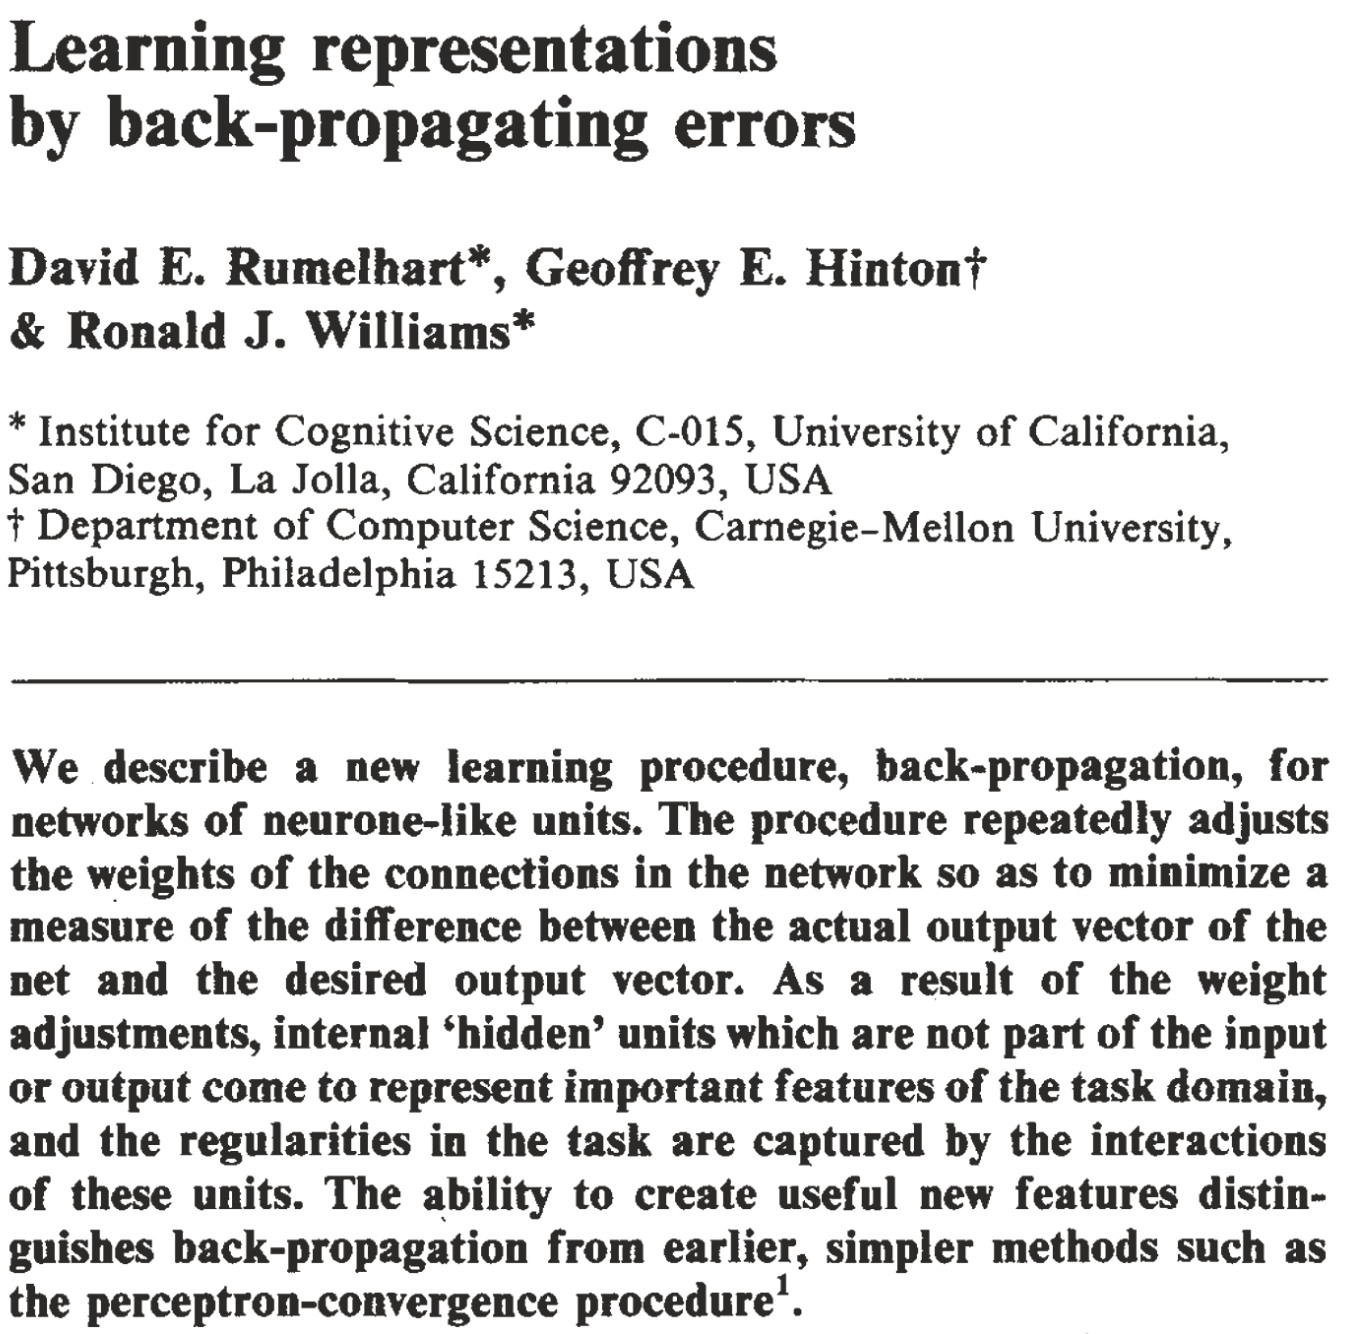
\includegraphics[width=6cm]{data/backprop.png}
            };
        }
        \visible<8>{
            \node[minimum width=2.1cm, minimum height=0.3cm, draw=red, thick] at (0.35, 1.8) {};
        }
        \visible<9-12>{
            \node[] (equation) at (0, -1.5) {
                $\Delta R(\theta^m)=\left.\dfrac{\partial \alert<11>{R(\alert<10>{\theta})}}{\partial \alert<10>{\theta}} \right|_{\alert<12>{\theta=\theta^m}}$
            };
            \node[anchor=north, text width=7cm, font=\footnotesize\selectfont] (where) at (equation.south) {
                \begin{itemize}
                    \item <10->$\theta$ are the parameters of the model
                    \item <11->$R(\theta)$ is the loss as a function of the parameters
                    \item <12->$\theta^m$ is a specific configuration of parameters
                \end{itemize}
            };
        }
        \visible<10>{
            \node[] at (0, 1.2) {
                \usebox{\lossparameters}
            };
        }
        \visible<11>{
            \node[] at (0, 1.2) {
                \usebox{\losssurface}
            };
        }
        \visible<12-13>{
            \node[] at (0, 1.2) {
                \usebox{\losspoint}
            };
        }
        \visible<13-15>{
            \node[] at (0, -2) {
                $\dfrac{\partial R_i(\theta)}{\partial w_{jk}} = \dfrac{\partial R(\theta)}{\partial f_\theta(x_i)} \cdot \dfrac{\partial f_\theta(x_i)}{\partial g(z_{ik})} \cdot \dfrac{\partial g(z_{ik})}{\partial z_{ik}} \cdot \dfrac{z_{ik}}{w_{kj}}$
            };
        }
        \visible<14>{
            \node[] at (0, 1.2) {
                \usebox{\lossdirection}
            };
        }
        \visible<15>{
            \node[] at (0, 1.2) {
                \usebox{\lossconvergence}
            };
        }
        \visible<16-17>{
            \node[text width=10cm] (gd) at (0, 0) {
                \underline{Backpropagation}: Uses gradient descent to iteratively determine how the model weights should be updated to minimize the loss function
                \begin{itemize}
                    \item \textbf{Gradient descent}: Calculate gradient based on all data points
                    \item <17> \textbf{Stochastic gradient descent}: Calculate gradient based on a batch of data points
                \end{itemize}
            };
        }
    \end{tikzpicture}
\end{frame}

\newsavebox{\tradeoff}
\sbox{\tradeoff}{
    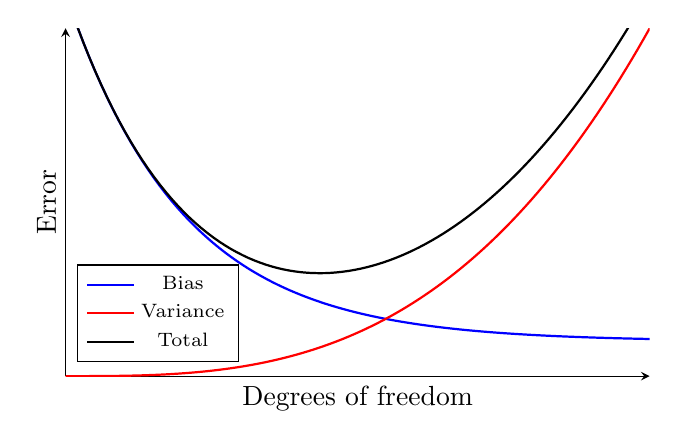
\begin{tikzpicture}
        \begin{axis}[
            height=6cm,
            width=9cm,
            xlabel={Degrees of freedom},
            axis x line*=bottom,
            axis y line*=left,
            axis line style={-stealth},
            xmajorticks=false,
            ymajorticks=false,
            xmin=0,
            xmax=1,
            ymin=0,
            ymax=1,
            ylabel=Error,
            legend style={at={(0.02, 0.04)}, font=\scriptsize\selectfont, align=left, anchor=south west}
        ]
            \addplot[blue, thick, domain=0:1, samples=100] (x, {exp(-5 * x) + 0.1});
            \addplot[red, thick, domain=0:1, samples=100] (x, x^3);
            \addplot[black, thick, domain=0:1, samples=100] (x, {exp(-5 * x) + 0.1 + x^3});
            %\addplot[red, smooth, thick] (x, x^2);
            \legend{Bias, Variance, Total}


        \end{axis}
    \end{tikzpicture}
}

\begin{frame}{Deep learning: The conundrum}
    \begin{tikzpicture}
        \node[] at (5.25, -3.5) {};
        \node[] at (-5.25, 3.5) {};

        \visible<1>{
            \node[] at (0, -1.2) {
                \usebox{\polynomialboth}
            };
        }
        \visible<1-3>{
            \node[text width=5cm, anchor=north west, font=\footnotesize\selectfont, text depth=0] at (-5.25, 3.25) {
                \underline{Splines}: A smooth curve implemented via piecewise polynomial functions
                \begin{itemize}
                    \item <2-> Requires us to carefully balance the complexity of the function
                \end{itemize}
            };
            \node[text width=5cm, anchor=north east, font=\footnotesize\selectfont, text depth=0] at (5.25, 3.26) {
                \underline{Neural networks}: A piecewise linear function implemented as a hierarchy of artificial neurons
                \begin{itemize}
                    \item <3> Overparameterization \emoji{partying-face}
                \end{itemize}
            };
        }
        \visible<4-5>{
            \node[] at (0, 0) {
                \usebox{\tradeoff}
            };
        }
        \visible<5>{
            \draw[gray!50, -stealth, line width=10pt] (-2, 0) -- (2, 0);
        }
        \visible<6>{
            \node[inner sep=0pt, draw=black] at (0, 1.75) {
                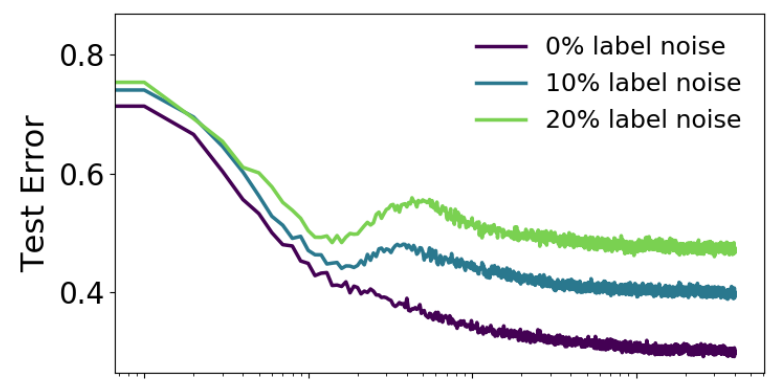
\includegraphics[width=6cm]{data/double_descent_epochs.png}
            };
            \node[inner sep=0pt, draw=black] at (0, -1.75) {
                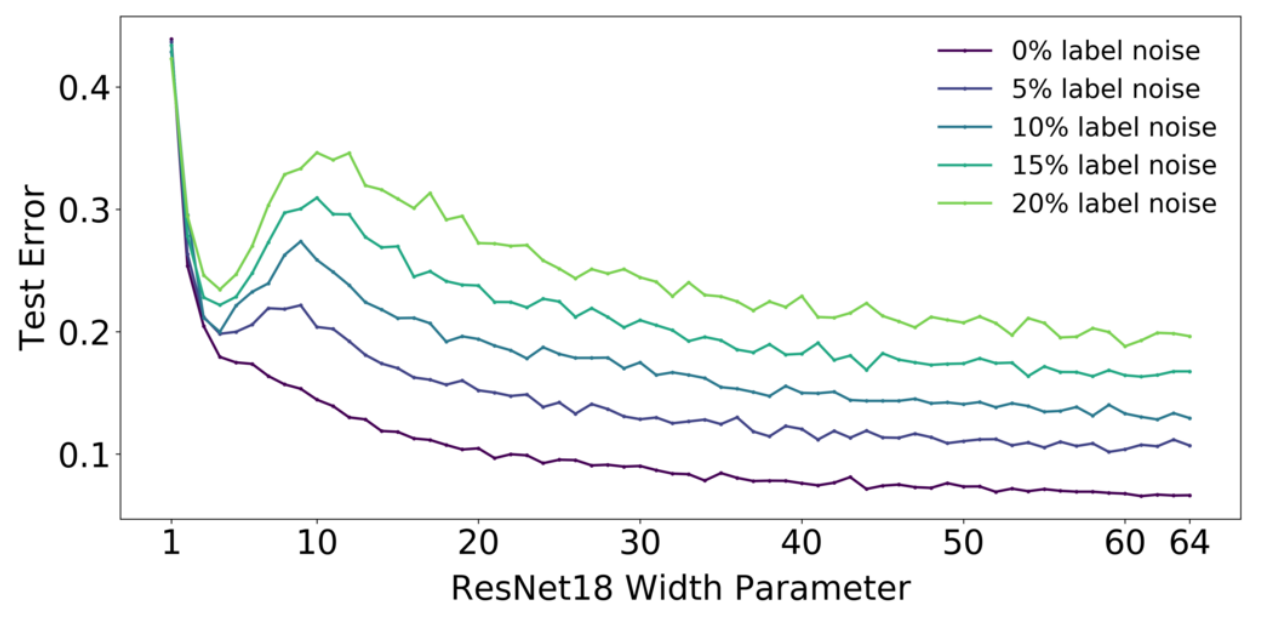
\includegraphics[width=6cm]{data/double_descent_width.png}
            };
        }
        \visible<7>{
            \node[inner sep=0pt, draw=black] at (0, 0) {
                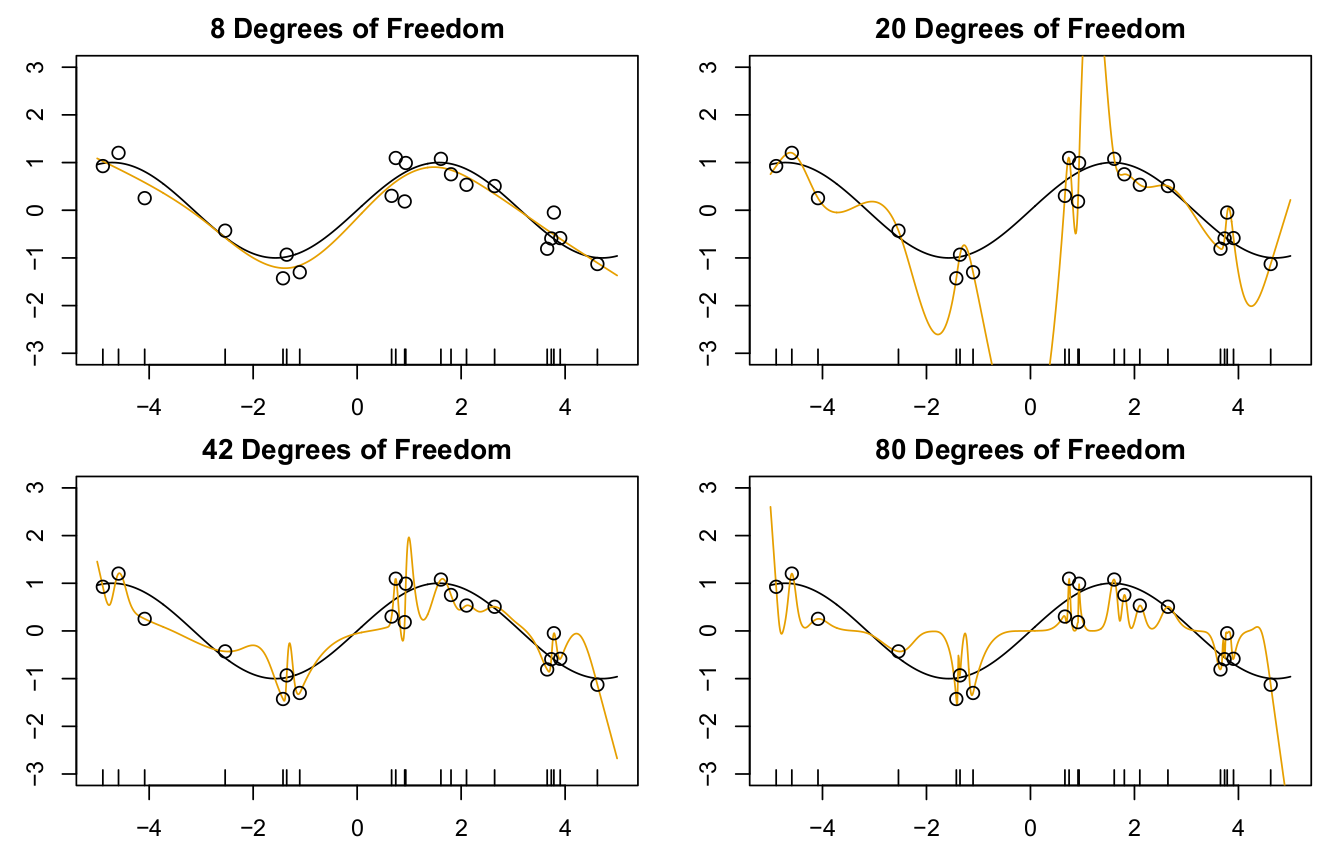
\includegraphics[width=9cm]{data/degrees_of_freedom.png}
            };
        }
        \visible<8>{
            \node[text width=10cm] at (0, 0) {
                \underline{Overparameterization}: Deep artificial neural networks generally have far more parameters than necessary (and often more than the number of data points)
                \begin{itemize}
                    \item At face value, it is surprising that this does not yield severe overfitting
                    \item However, it can be shown that neural networks, after perfectly fitting their training data, generally become more well-behaved and less wild
                \end{itemize}
            };
        }
    \end{tikzpicture}
\end{frame}

\begin{frame}{Deep learning: Regularization}
    \begin{tikzpicture}
        \node[] at (-5.25, 3.5) {};
        \node[] at (5.25, -3.5) {};

        \node[text width=10cm] at (0, 2) {
            \begin{itemize}
                \item \underline{Weight decay}: Applies an $\ell_2$-penalty to the weights, similarly to ridge regression
                \item[] $R(\theta;\lambda) = R(\theta) + \lambda \sum \theta^2$
                \item <2-> \underline{Dropout}: Randomly kills a fraction of the neurons during training
                \item <10-> \underline{Data augmentation}: Attempts to generate more data
            \end{itemize}
        };
        \visible<3-9>{
            \artificialneuron{(-2, -0.25)}{n00}{0}
            \artificialneuron{(-2, -1)}{n01}{0}
            \artificialneuron{(-2, -1.75)}{n02}{0}
            \artificialneuron{(-2, -2.5)}{n03}{0}

            \artificialneuron{(0, -0.625)}{n10}{0}
            \artificialneuron{(0, -1.375)}{n11}{0}
            \artificialneuron{(0, -2.125)}{n12}{0}

            \artificialneuron{(2, -1.375)}{n20}{0}

            \draw[-stealth] (n00) -- (n10);
            \draw[-stealth] (n00) -- (n11);
            \draw[-stealth] (n00) -- (n12);
            \draw[-stealth] (n01) -- (n10);
            \draw[-stealth] (n01) -- (n11);
            \draw[-stealth] (n01) -- (n12);
            \draw[-stealth] (n02) -- (n10);
            \draw[-stealth] (n02) -- (n11);
            \draw[-stealth] (n02) -- (n12);
            \draw[-stealth] (n03) -- (n10);
            \draw[-stealth] (n03) -- (n11);
            \draw[-stealth] (n03) -- (n12);

            \draw[-stealth] (n10) -- (n20);
            \draw[-stealth] (n11) -- (n20);
            \draw[-stealth] (n12) -- (n20);
        }

        \visible<4-5>{
            \node[inner sep=0pt, draw=black] (cat) at (-4, -0.25) {
                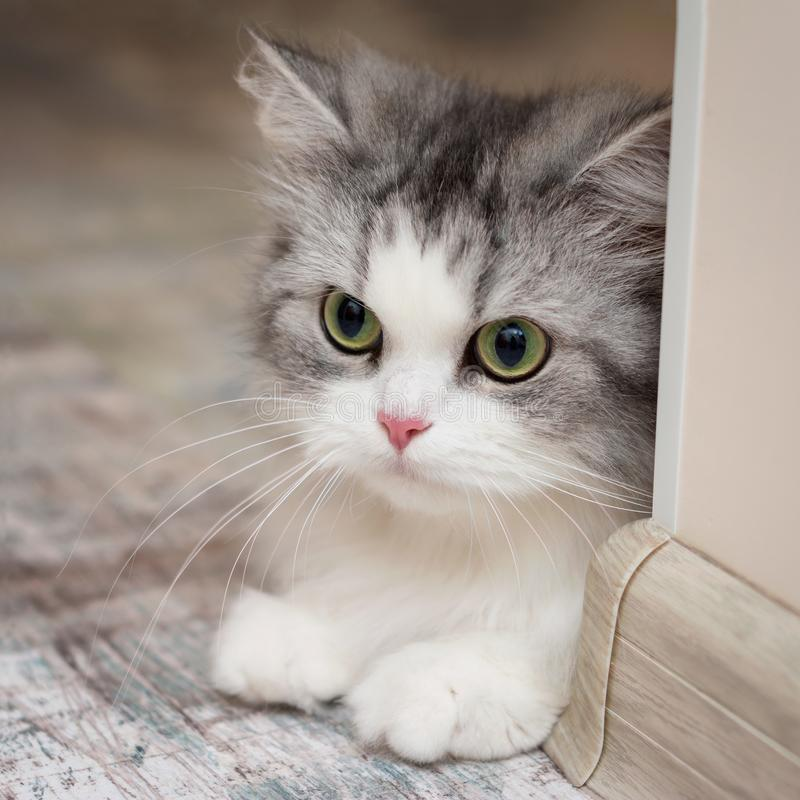
\includegraphics[width=1cm]{data/cat.png}
            };
            \node[inner sep=0pt, draw=black] (dog) at (-4, -1.375) {
                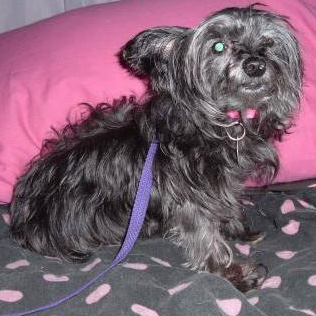
\includegraphics[width=1cm]{data/dog.jpg}
            };
            \node[inner sep=0pt, draw=black] (shark) at (-4, -2.5) {
                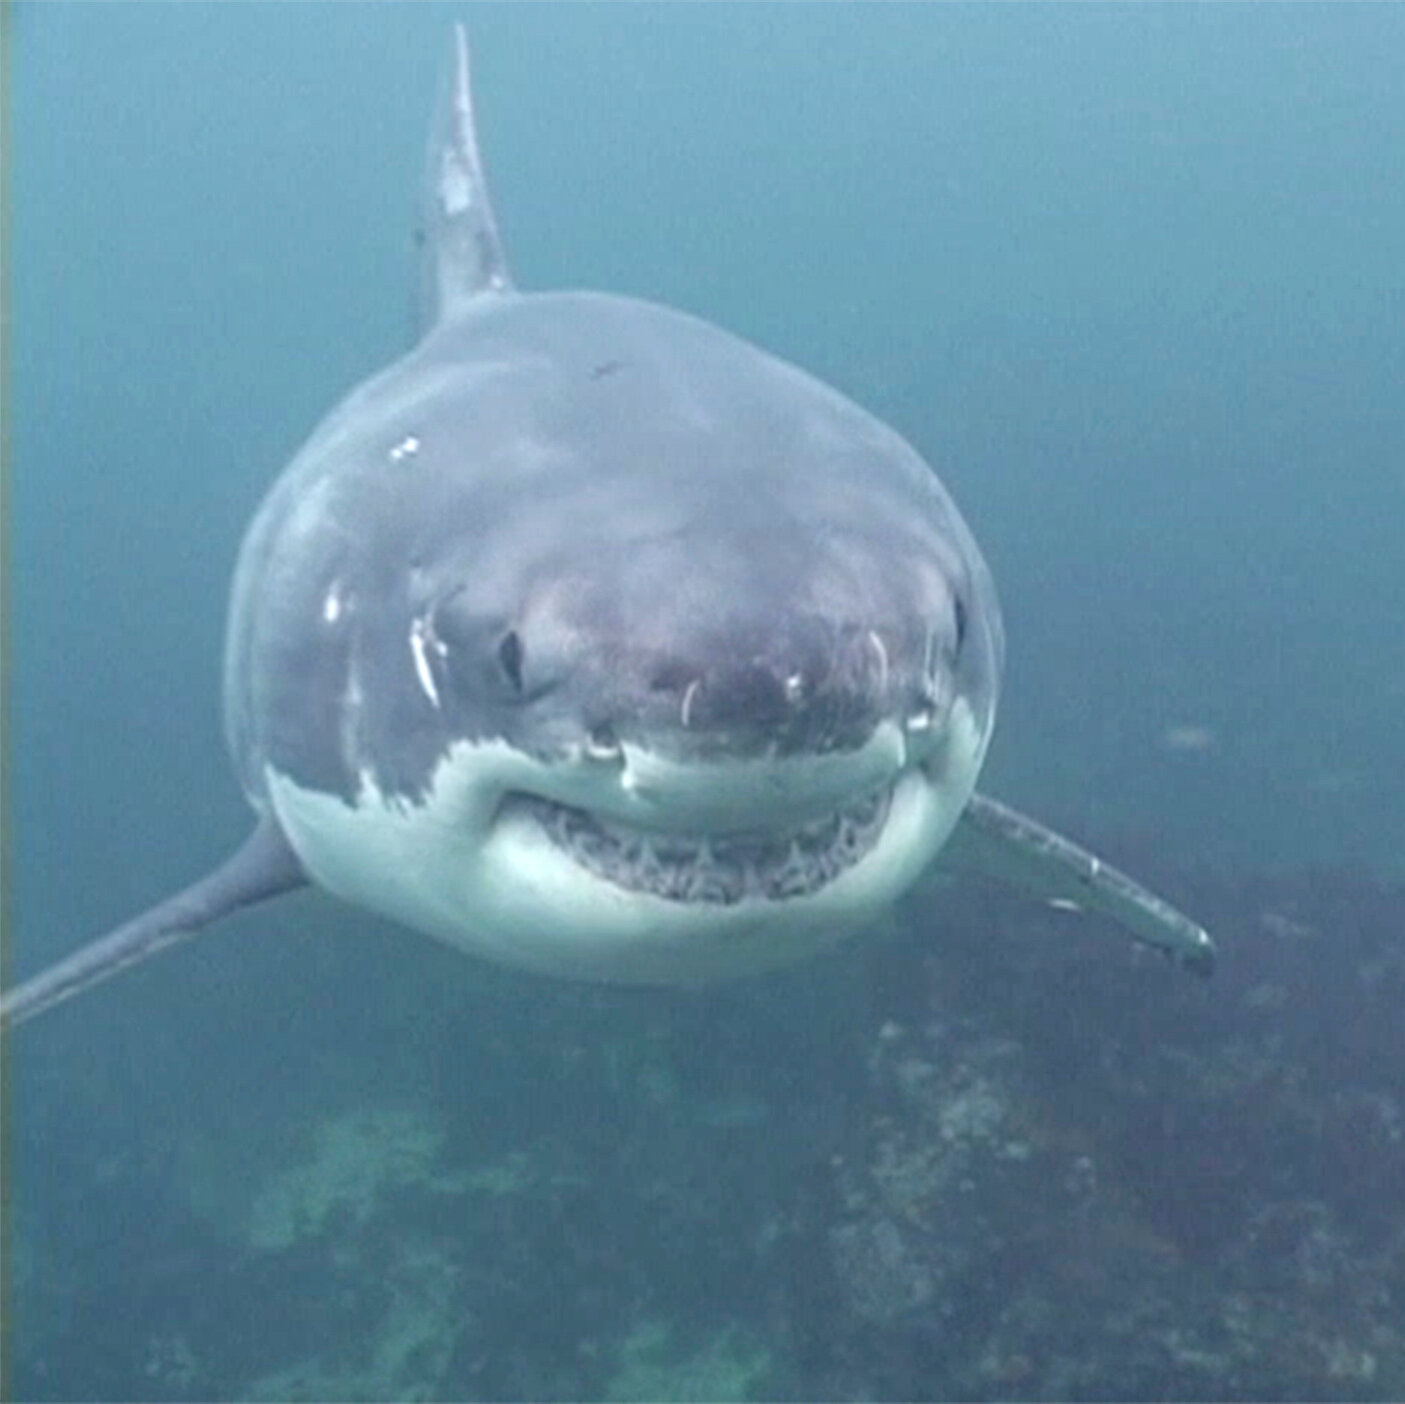
\includegraphics[width=1cm]{data/shark.jpeg}
            };

            \draw[-stealth] (cat) -- (n00);
            \draw[-stealth] (cat) -- (n01);
            \draw[-stealth] (cat) -- (n02);
            \draw[-stealth] (cat) -- (n03);

            \draw[-stealth] (dog) -- (n00);
            \draw[-stealth] (dog) -- (n01);
            \draw[-stealth] (dog) -- (n02);
            \draw[-stealth] (dog) -- (n03);

            \draw[-stealth] (shark) -- (n00);
            \draw[-stealth] (shark) -- (n01);
            \draw[-stealth] (shark) -- (n02);
            \draw[-stealth] (shark) -- (n03);
        }
        \visible<5-7>{
            \begin{scope}
                \clip (0, -0.625) circle (0.24cm) node {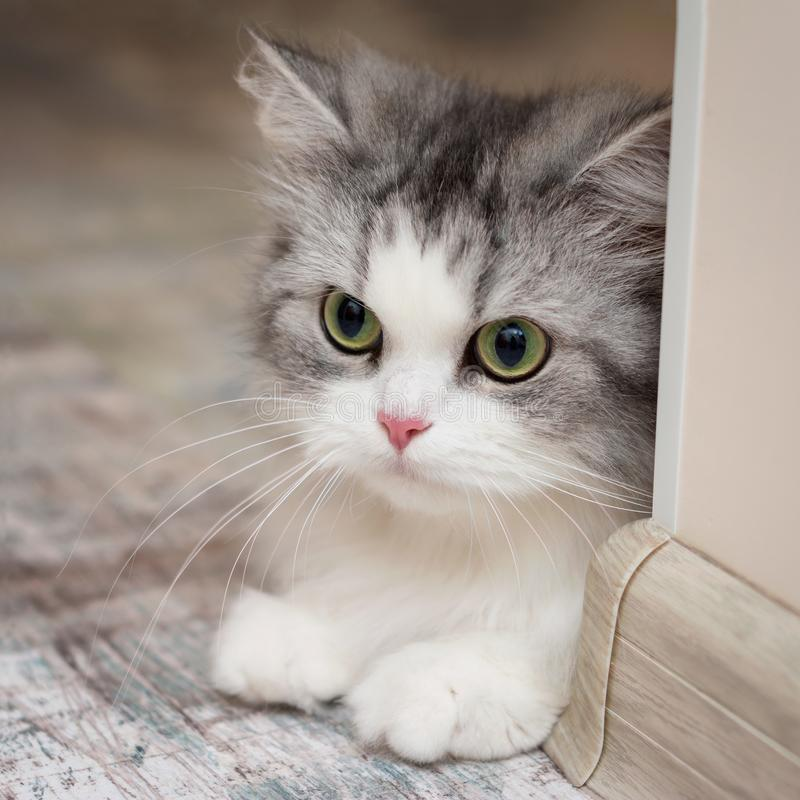
\includegraphics[width=14pt]{data/cat.png}};
            \end{scope}
            \begin{scope}
                \clip (0, -1.375) circle (0.24cm) node {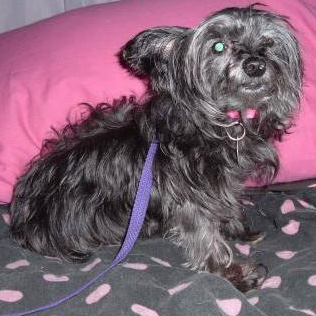
\includegraphics[width=14pt]{data/dog.jpg}};
            \end{scope}
            \begin{scope}
                \clip (0, -2.125) circle (0.24cm) node {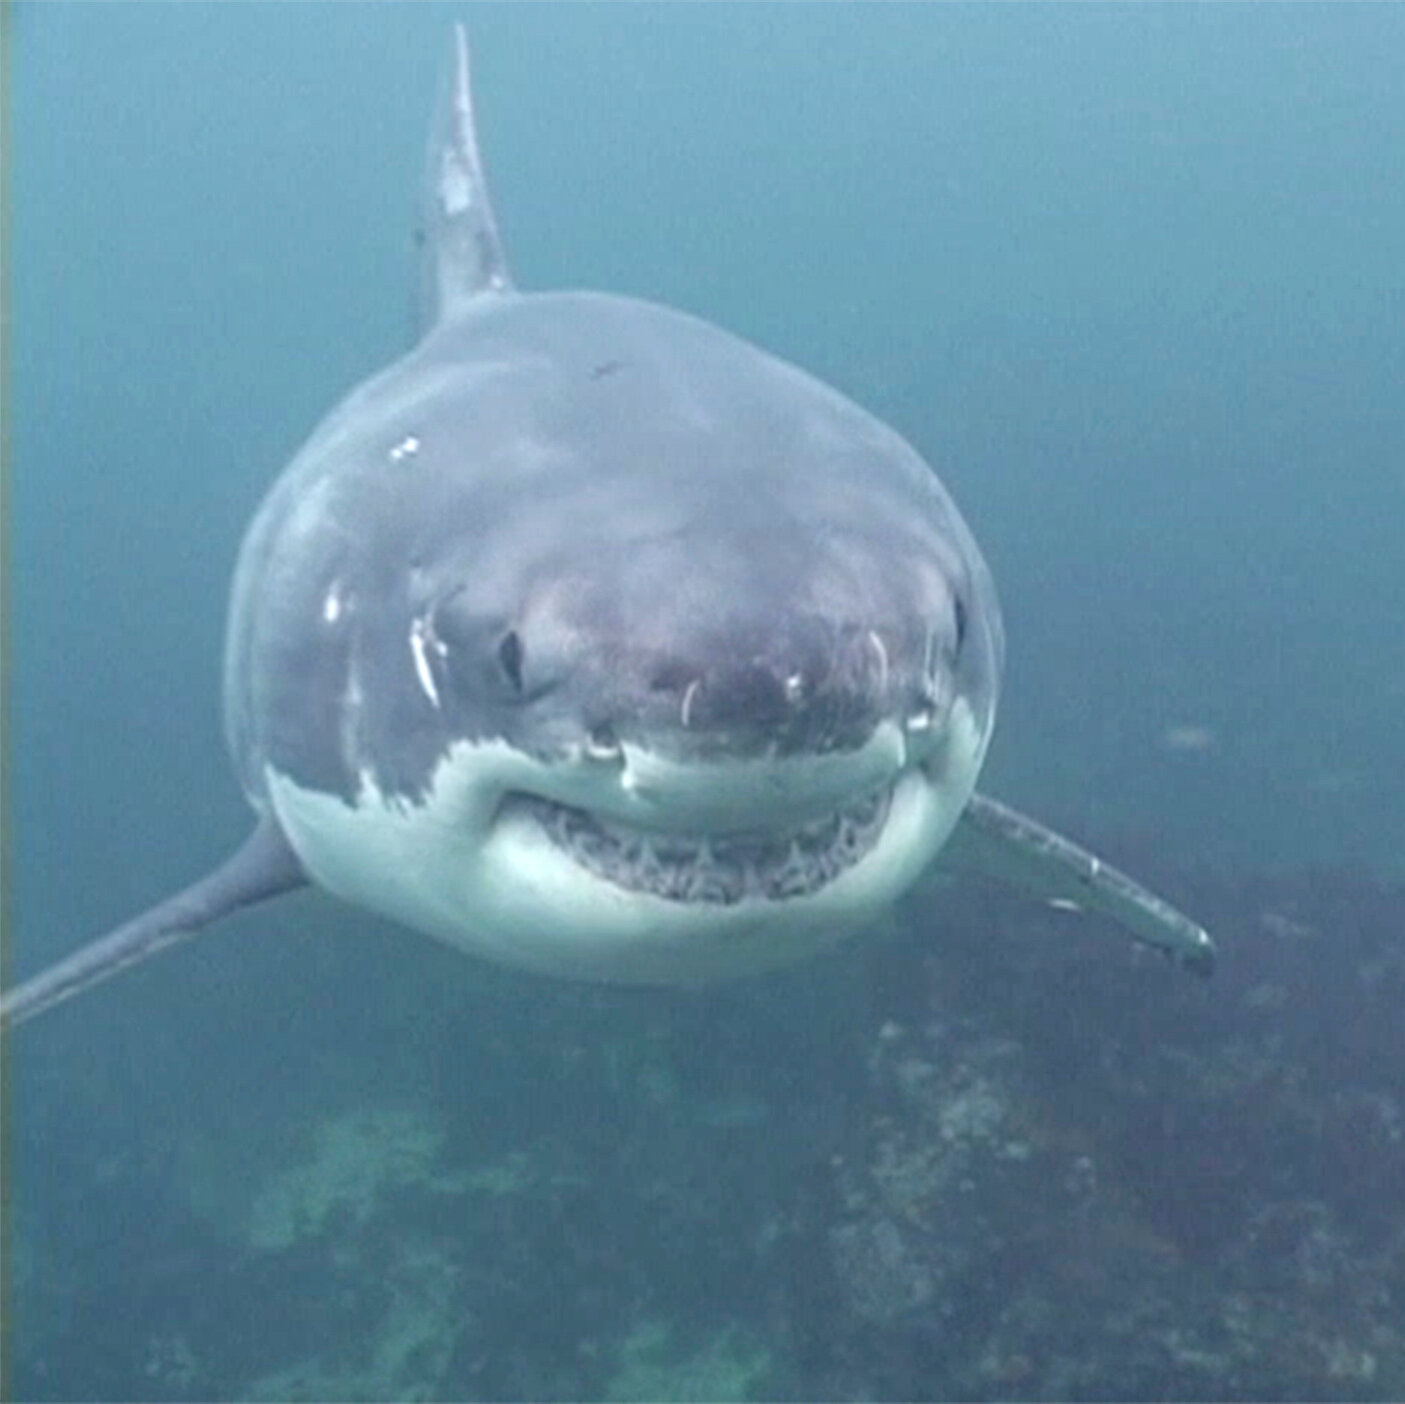
\includegraphics[width=14pt]{data/shark.jpeg}};
            \end{scope}
        }
        \visible<6>{
            \node[inner sep=0pt, draw=black] (cat) at (-4, -1.375) {
                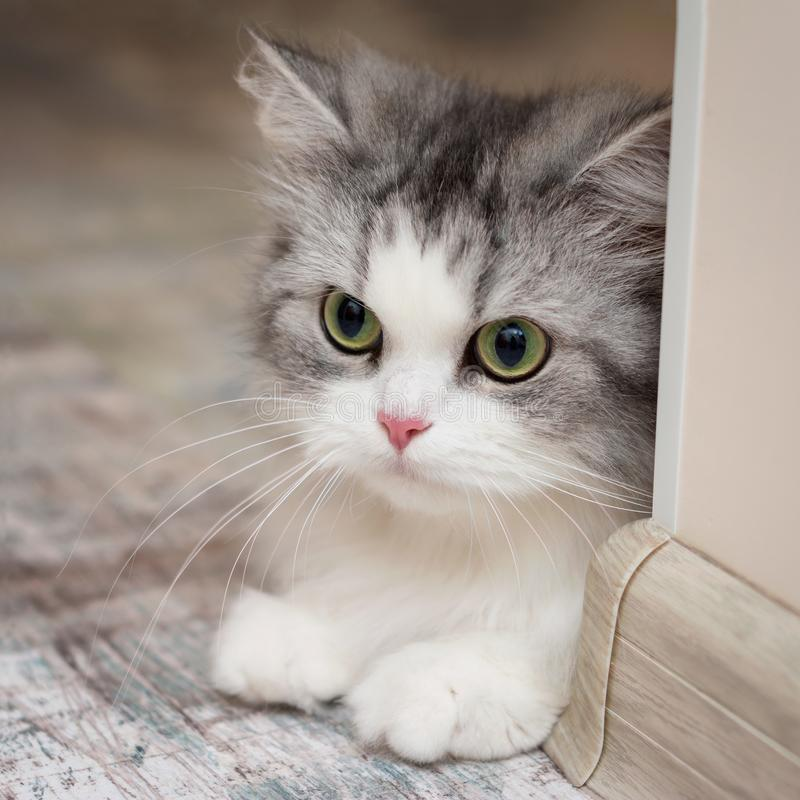
\includegraphics[width=1cm]{data/cat.png}
            };

            \draw[-stealth, red] (cat) -- (n00);
            \draw[-stealth, red] (cat) -- (n01);
            \draw[-stealth, red] (cat) -- (n02);
            \draw[-stealth, red] (cat) -- (n03);

            \draw[-stealth, red] (n00) -- (n10);
            \draw[-stealth, red] (n01) -- (n10);
            \draw[-stealth, red] (n02) -- (n10);
            \draw[-stealth, red] (n03) -- (n10);

            \draw[-stealth, red] (n10) -- (n20);

            \node[text=red, anchor=west] at ($ (n20.east) $) {
                Cat
            };
        }
        \visible<7>{
            \node[inner sep=0pt, draw=black] (cat) at (-4, -1.375) {
                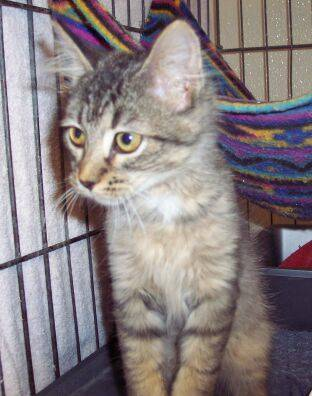
\includegraphics[width=1cm]{data/other_cat.jpg}
            };

            \draw[-stealth, red] (cat) -- (n00);
            \draw[-stealth, red] (cat) -- (n01);
            \draw[-stealth, red] (cat) -- (n02);
            \draw[-stealth, red] (cat) -- (n03);

            \node[anchor=west] at ($ (n20.east) $) {
                ?
            };
        }
        \visible<8>{
            \node[inner sep=0pt, draw=black] (cat) at (-4, -1.375) {
                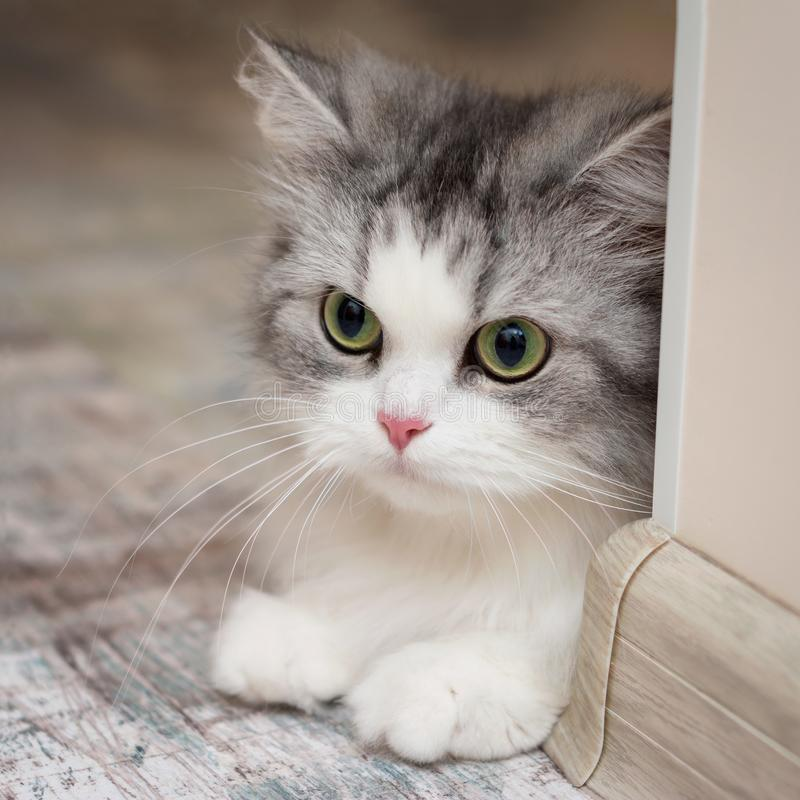
\includegraphics[width=1cm]{data/cat.png}
            };

            \draw[-stealth] (cat) -- (n00);
            \draw[-stealth] (cat) -- (n01);
            \draw[-stealth] (cat) -- (n02);
            \draw[-stealth] (cat) -- (n03);

            \node[
                circle,
                draw=black,
                fill=gray!50,
                minimum size=\nodesize,
                inner sep=0pt
            ] at (-2, -1.75) {};
            \node[
                circle,
                draw=black,
                fill=gray!50,
                minimum size=\nodesize,
                inner sep=0pt
            ] at (0, -0.625) {};
        }
        \visible<9>{
            \node[inner sep=0pt, draw=black] (cat) at (-4, -1.375) {
                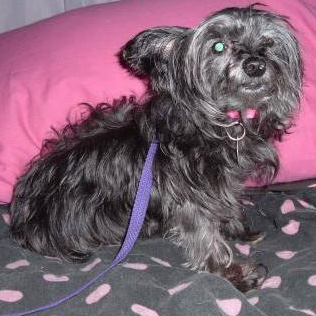
\includegraphics[width=1cm]{data/dog.jpg}
            };

            \draw[-stealth] (cat) -- (n00);
            \draw[-stealth] (cat) -- (n01);
            \draw[-stealth] (cat) -- (n02);
            \draw[-stealth] (cat) -- (n03);

            \node[
                circle,
                draw=black,
                fill=gray!50,
                minimum size=\nodesize,
                inner sep=0pt
            ] at (-2, -1.00) {};
            \node[
                circle,
                draw=black,
                fill=gray!50,
                minimum size=\nodesize,
                inner sep=0pt
            ] at (0, -2.125) {};
        }
    \end{tikzpicture}
\end{frame}
